\documentclass[aspectratio=169,10pt]{beamer}

\usepackage[utf8]{inputenc}
\usepackage{graphicx}
\usepackage{booktabs}
\usepackage{tabularx}
\usepackage{amsmath}
\usepackage{subcaption}
\usepackage{pifont}
\usepackage{tikz}
\usetikzlibrary{arrows.meta,positioning}
\usepackage{grffile}

\newcommand{\cmark}{\ding{51}}
\newcommand{\xmark}{\ding{55}}

\usetheme{Madrid}
\usecolortheme{seahorse}
\setbeamertemplate{navigation symbols}{}
\setbeamertemplate{caption}[numbered]
\setbeamerfont{caption}{size=\tiny}
\setbeamercolor{block title}{bg=blue!20,fg=black}
\setbeamercolor{block body}{bg=blue!5,fg=black}

\title[Cache Reverse Engineering]{Predicting Cache Evolution: The Growing Capacity and Latency Cost of CPU Caching}
\author{Nick Ngo \and Kevin Chen}
\institute{ECE 592 -- Fall 2026}
\date{}

\begin{document}

% ============================================================
\begin{frame}
\titlepage
\end{frame}

% ============================================================
\begin{frame}{Motivation and Experimental Question}
\textbf{Question:} Can a cache hierarchy's geometry, latency, and inclusion behavior be
reverse engineered from timing alone, and does that hierarchy change predictably across
CPU generations and vendors?

\medskip
\begin{block}{Three-phase discipline (non-negotiable)}
\begin{enumerate}
    \item \textbf{Phase I -- timing only:} no PMU, no cache-topology files, no vendor tables.
    \item \textbf{Phase II -- counter \& literature verification:} \texttt{perf}, \texttt{lscpu}, Agner Fog / vendor docs.
    \item \textbf{Phase III -- Hazel:} a lab-only prediction is frozen \emph{before} touching the held-out HPC cluster.
\end{enumerate}
\end{block}

\medskip
Six timing-only targets: cache-level/capacity, line size, associativity, hit latency,
miss/next-level latency, inclusion/exclusion -- one shared, portable benchmark binary
(\texttt{cache\_bench}) implements all six.
\end{frame}

% ============================================================
\begin{frame}{Experimental Platforms: 8 Lab Machines + Hazel}
\centering\scriptsize
\begin{tabular}{lllll}
\toprule
Machine & Vendor/ISA & Microarch. & Year & Node \\
\midrule
Sunbird & Intel x86-64 & Haswell & 2014 & 22\,nm \\
Charnwood & Intel x86-64 & Skylake & 2015 & 14\,nm \\
Ookay & Intel x86-64 & Kaby Lake & 2017 & 14\,nm \\
Upgrade & Intel x86-64 & Coffee Lake & 2017 & 14\,nm \\
Crux & Intel x86-64 & Coffee Lake Refresh & 2019 & 14\,nm \\
Skylark & AMD x86-64 & Zen 2 & 2019 & 7\,nm \\
Thunderbird & Ampere AArch64 & Neoverse N1 & 2020 & 7\,nm \\
Artemisia & Intel x86-64 & Sapphire Rapids & 2023 & 10\,nm \\
\midrule
Hazel-Haswell & Intel x86-64 (HPC) & Haswell-EP & 2014 & 22\,nm \\
\bottomrule
\end{tabular}

\vspace{4mm}
\textbf{Coverage:} 2014--2023, 3 vendors (Intel/AMD/Ampere), 2 ISAs (x86-64/AArch64),
desktop + server class, plus 1 held-out Slurm HPC generation.
\end{frame}

% ============================================================
\begin{frame}{Shared Measurement Infrastructure}
\begin{columns}[T]
\column{0.5\textwidth}
\textbf{Dependent pointer-chase primitive}
\begin{itemize}
    \item Singly-linked cycle of fixed-size nodes; load $i{+}1$'s address is the \emph{value} of load $i$
    \item Forces true load-to-use latency -- no reorder/prefetch across the chain
    \item Serialized cycle counters: \texttt{LFENCE+RDTSC(P)} (x86), \texttt{DSB+ISB+CNTVCT\_EL0} (ARM)
\end{itemize}
\column{0.5\textwidth}
\textbf{Batching \& controls}
\begin{itemize}
    \item Batches of 1000 accesses amortize timer overhead; $\geq$1{,}000{,}000 timed accesses/point
    \item Every sweep run at \emph{random} (chase) \textbf{and} \emph{sequential} (prefetcher control) patterns
    \item Independent-load timer exposes MLP as a sanity check on the dependent chain
\end{itemize}
\end{columns}
\medskip
One binary, \texttt{cache\_bench}, dispatches all six experiments via \texttt{--experiment};
identical code runs unmodified on x86-64 and AArch64.
\end{frame}

% ============================================================
\begin{frame}{Result: Capacity / Cache-Level Discovery}
\begin{columns}[T]
\column{0.55\textwidth}
\centering
\includegraphics[width=\linewidth]{flow_capacity.png}
\column{0.45\textwidth}
\centering
\includegraphics[width=\linewidth]{sunbird_capacity.png}
\end{columns}
\begin{block}{Finding}
A reproducible, sustained step in random-pattern ticks/access (absent on the sequential
control) marks a level boundary; L1D/L2 matched PMU exactly on all 8 machines, LLC on 5/8.
\end{block}
\end{frame}

% ============================================================
\begin{frame}{Result: Cache Line Size}
\begin{columns}[T]
\column{0.55\textwidth}
\centering
\includegraphics[width=\linewidth]{flow_linesize.png}
\column{0.45\textwidth}
\centering
\includegraphics[width=\linewidth]{sunbird_linesize.png}
\end{columns}
\begin{block}{Finding}
Two independently designed methods (stride-saturation and footprint-family) agree at
\textbf{64\,B on 8 of 8 machines} -- the single most consistent result in the project
(one exception: Skylark's LLC region measures 128\,B by both methods).
\end{block}
\end{frame}

% ============================================================
\begin{frame}{Result: Cache Associativity -- and an Honest Negative Result}
\begin{columns}[T]
\column{0.55\textwidth}
\centering
\includegraphics[width=\linewidth]{flow_assoc.png}
\column{0.45\textwidth}
\centering
\includegraphics[width=\linewidth]{sunbird_assoc_L1.png}
\end{columns}
\begin{block}{Finding}
L1 associativity is confirmed cleanly everywhere (8-way x86, 4-way ARM). \textbf{L2/LLC are
blocked by a real confound}: byte-capacity candidates spanning up to 32$\times$ break at the
\emph{same} small num\_ways ($\approx$9--10) regardless of capacity -- a shared,
capacity-independent structure (leading hypothesis: DTLB aliasing), not real cache signal.
\end{block}
\end{frame}

% ============================================================
\begin{frame}{Result: Cache Hit Latency}
\begin{columns}[T]
\column{0.5\textwidth}
\centering
\includegraphics[width=\linewidth]{flow_hitlat.png}
\column{0.5\textwidth}
\centering

\includegraphics[width=0.48\linewidth]{sunbird_hitlat_L1.png}\hfill

\includegraphics[width=0.48\linewidth]{sunbird_hitlat_L2.png}\\[2pt]

\includegraphics[width=0.48\linewidth]{sunbird_hitlat_LLC.png}\hfill

\includegraphics[width=0.48\linewidth]{sunbird_hitlat_DRAM.png}
\end{columns}
\begin{block}{Finding}
Dependent/random median at a confirmed single-level footprint, validated by an
independent-load control reading faster at every level -- Sunbird: a clean monotonic
10.4 / 26.8 / 58.4 / 207\,tick ladder (L1/L2/LLC/DRAM).
\end{block}
\end{frame}

% ============================================================
\begin{frame}{Result: Miss / Next-Level Latency}
\begin{columns}[T]
\column{0.5\textwidth}
\centering
\includegraphics[width=\linewidth]{flow_misslat.png}
\column{0.5\textwidth}
\centering

\includegraphics[width=0.32\linewidth]{sunbird_misslat_L1_to_L2.png}

\includegraphics[width=0.32\linewidth]{sunbird_misslat_L2_to_LLC.png}

\includegraphics[width=0.32\linewidth]{sunbird_misslat_LLC_to_DRAM.png}
\end{columns}
\begin{block}{Finding}
Single-shot reload after an untimed eviction walk gives an increasing 124/284/622-tick
sequence (Sunbird) -- but single-shot timing carries a fixed $\approx$64--85 tick overhead
(isolated via a control eviction set), so this is reload latency \emph{plus} overhead, not
a clean incremental number.
\end{block}
\end{frame}

% ============================================================
\begin{frame}{Result: Inclusion and Exclusion Behavior}
\begin{columns}[T]
\column{0.55\textwidth}
\centering
\includegraphics[width=\linewidth]{flow_inclusion.png}
\column{0.45\textwidth}
\centering
\includegraphics[width=\linewidth]{sunbird_incl_L1_vs_L2.png}
\end{columns}
\begin{block}{Finding}
A page-offset eviction walk structurally avoids the target's own upper-level set;
classifying reload latency against survived/invalidated calibration gives
\textbf{L1 vs.\ L2 non-inclusive on 6 of 8 machines} -- the one pairing that reproduces
consistently. LLC-involving pairings show no fleet-wide agreement (Section~8, caveat:
an L2 target's index does not fit in one page).
\end{block}
\end{frame}

% ============================================================
\begin{frame}{Phase II: Performance Counter Verification}
\centering\scriptsize
\begin{tabular}{lccccl}
\toprule
Machine & L1D size & L1D assoc. & L2 assoc. & LLC size & LLC assoc.\\
\midrule
Sunbird & \cmark & \cmark & \cmark & \cmark & \xmark~(20w)\\
Charnwood & \cmark & \cmark & \xmark~(4w) & \cmark & \xmark~(16w)\\
Ookay & \cmark & \cmark & \xmark~(4w) & \cmark & \xmark~(16w)\\
Upgrade & \cmark & \cmark & \xmark~(4w) & \cmark & \xmark~(16w)\\
Crux & \cmark & \cmark & \xmark~(4w) & \xmark~(1.5x) & \xmark~(12w)\\
Skylark & \cmark & \cmark & \cmark & \xmark~(2x) & \xmark~(16w)\\
Thunderbird & \cmark & \cmark & \xmark~(8w) & n/a & lit.\ 16w\\
Artemisia & \cmark & \cmark & \cmark & \xmark~(1.75x) & \xmark~(15w, close)\\
\bottomrule
\end{tabular}

\medskip
\begin{block}{Headline}
\textbf{L1D matched ground truth on 8 of 8 machines, zero exceptions} -- the strongest
validation in the project. The confound-blocked L2/LLC associativity guess was right on
only 3/8 and 1/8 machines respectively, confirming Section~4's own low-confidence flag.
\end{block}
\end{frame}

% ============================================================
\begin{frame}{Eight Performance Counters Across Generations}
\centering

\includegraphics[width=0.85\linewidth]{eightcounters_latency_scurve.png}
\begin{block}{Finding}
Per-access latency ranked ascending, colored by vendor: Intel machines cluster
tightest; Skylark (AMD) shows a striking dTLB-miss anomaly (2--4 orders of magnitude
lower than every other machine at LLC/beyond-LLC footprints) -- a real architectural
TLB-reach difference, reproducible across two benchmark tiers.
\end{block}
\end{frame}

% ============================================================
\begin{frame}{Software-Only Cache Hit-Rate Metric}
\begin{columns}[T]
\column{0.5\textwidth}
\centering
\includegraphics[width=\linewidth]{flow_hitrate.png}
\column{0.5\textwidth}
\centering
\includegraphics[width=0.95\linewidth]{chrono_14_software_hit_rate.png}
\end{columns}
\begin{block}{Finding}
A single self-calibrated latency threshold + Rogan--Gladen debiasing detects
L1/L2-scale residency well (10--20\% median PMU relative error) but \textbf{fails at
LLC/DRAM scale} (60--100\% error) -- a disclosed single-threshold limitation, not a bug
found after the fact. At a standardized 256\,KiB workload, 7 of 8 machines read
$\approx$1.0; only Sunbird is a statistically real outlier (a boundary/conflict effect).
\end{block}
\end{frame}

% ============================================================
\begin{frame}{Cache Evolution: Moore-Style Trends}
\centering

\includegraphics[width=0.48\linewidth]{chrono_05_l2_capacity.png}\hfill

\includegraphics[width=0.48\linewidth]{chrono_11_llc_latency_and_miss_penalty.png}
\begin{block}{Finding}
Per-core L2 capacity grows in a genuine, if \emph{step-wise} (not smooth), doubling
pattern: flat at 256\,KiB for 5 years, then three back-to-back doublings in 4 years.
LLC hit latency does \textbf{not} track LLC capacity monotonically -- topology
(interconnect, core count) dominates once sharing-domain differences are PMU-corrected.
\end{block}
\end{frame}

% ============================================================
\begin{frame}{Our Laws: Frozen Predictions vs.\ Held-Out Hazel}
\centering

\includegraphics[width=0.48\linewidth]{law1_l2_capacity_heldout.png}\hfill

\includegraphics[width=0.48\linewidth]{law2_l1d_invariance_heldout.png}
\begin{block}{Finding}
\footnotesize
\textbf{Law 1 (Doubling):} $C(t) = 256\,\text{KiB}\cdot 2^{(t-2014)/3}$, fit Sunbird 2014
$\to$ Artemisia 2023 ($8\times$ over 9 years, step-wise not smooth). Dashed line = frozen
extrapolation to 2028 ($\sim$6.35\,MiB). Hazel's own L2 boundary never resolved --
\textbf{untestable this pass}.\\[2pt]
\textbf{Law 2 (Invariance):} L1D capacity/assoc./line size constant across a decade, 3
vendors (32,768\,B / 8-way / 64\,B, 6 of 8 machines); dashed line reverts to that
majority value, not a fit through Artemisia's outlier. Hazel-Haswell (star) matched
exactly -- \textbf{supported}.
\end{block}
\end{frame}

% ============================================================
\begin{frame}{Hazel Held-Out Validation}
\centering
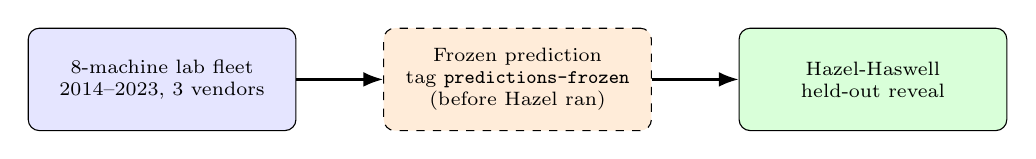
\begin{tikzpicture}[
    box/.style={draw, rounded corners, align=center, minimum height=1.3cm, minimum width=3.4cm, font=\scriptsize},
    arr/.style={-{Latex[length=2.5mm]}, thick}
]
\node[box, fill=blue!10] (lab) {8-machine lab fleet\\2014--2023, 3 vendors};
\node[box, fill=orange!15, dashed, right=1.1cm of lab] (freeze) {Frozen prediction\\tag \texttt{predictions-frozen}\\(before Hazel ran)};
\node[box, fill=green!15, right=1.1cm of freeze] (hazel) {Hazel-Haswell\\held-out reveal};
\draw[arr] (lab) -- (freeze);
\draw[arr] (freeze) -- (hazel);
\end{tikzpicture}

\vspace{3mm}
\centering\tiny
\begin{tabular}{llll}
\toprule
Quantity & Frozen prediction & Hazel measured & Verdict\\
\midrule
L1D capacity/assoc./line size & 32,768\,B / 8-way / 64\,B & exact match, all 3 & \textbf{Supported}\\
LLC capacity & $\sim$31.46\,MB & $\sim$22--24\,MB & Weakened ($\sim$25--30\% low, SKU effect)\\
L2 capacity/assoc. & 256\,KiB / 8-way & no clean boundary & Untestable this pass\\
Inclusion, L1 vs.\ LLC (skip-level) & lean inclusive & non-inclusive & \textbf{Falsified}\\
\bottomrule
\end{tabular}

\medskip
8 of 15 predicted quantities cleanly supported; a genuinely mixed, honestly reported result.
\end{frame}

% ============================================================
\begin{frame}{Limitations and Contributions}
\begin{columns}[T]
\column{0.5\textwidth}
\textbf{Limitations}
\begin{itemize}
    \item L2/LLC associativity unresolved by timing alone above L1 (shared confound)
    \item Miss-latency single-shot overhead not auto-subtracted
    \item Software hit-rate estimator: L1/L2-scale only, fails at LLC/DRAM
    \item Hazel: full suite on 1 of 9 available generations (haswell); Phase II not yet run there
\end{itemize}
\column{0.5\textwidth}
\textbf{Contributions}
\begin{itemize}
    \item Nick Ngo: capacity/associativity/latency/inclusion engines, all lab sweeps, PMU verification (6 machines), chronological analysis \& cache laws
    \item Kevin Chen: line-size engine (both methods), software hit-rate estimator, timer/portability layer, eight-counter study, entire Hazel HPC pipeline
\end{itemize}
\end{columns}

\bigskip
\centering\textbf{Conclusion:} L1D geometry is the one part of the memory hierarchy that
has not needed to change across a decade and three competing vendors.
\end{frame}

\end{document}
